\begin{center}
    \textsc{\Large\textbf{Locus of a Point}}
\end{center}

\begin{center}
    \begin{tikzpicture}
        \tzcoor*(0, 0)(O)
        \foreach \A in {0, 20,..., 340}{
            \tzdot*(\A:2)
            \tzline[dashed](O)(\A:2)
            \tzline[->](\A:2)(\A + 10:2)
        }
    \end{tikzpicture}
\end{center}


\begin{quote}
    Imagine you're at a park with a beautiful fountain at the center. You and your friend decide to play a game where you always stay exactly 10 feet away from the fountain.

    You start walking, keeping that distance constant. As you move around the fountain, you notice your feet are tracing a perfect circle with the fountain at the center. This path your feet are creating is called the \textbf{locus}.

    In geometry, a locus is the set of all points that satisfy a specific condition. In this game, the locus is the circle formed by your feet always being 10 feet from the fountain.

    So, the locus is just a fancy way of describing the path or shape created by a point (in this case, your feet) moving according to certain rules.
\end{quote}

\begin{quote}
    \textit{
        A locus is essentially the path traced out by a moving point that moves according to a specific set of conditions or rules.
    }
\end{quote}

\vspace*{10mm}

\begin{center}
    \textsc{\large Equation of a Line}
\end{center}

\begin{quote}
    \textit{
        A line can be defined as the locus of a point that moves in such a way that it maintains a constant rate of change between its coordinates. This constant rate of change is known as the slope. \\[2mm]
    }
\end{quote}

\begin{center}
    \begin{tikzpicture}
        \tzcoor*(2, 2)(P){$P(x_1, y_1)$}[al]
        \tzcoor*(5, 4)(Q){$Q(x_2, y_2)$}[al]
        \tzcoor*($0.5*(P) + 0.5*(Q)$)(M){$M(x, y)$}[al]
        \tzLFn(P)(Q)[1:6]
    \end{tikzpicture}
\end{center}

\begin{quote}
    Consider two fixed points \( P(x_1, y_1) \) and \( Q(x_2, y_2) \) and a moving point \( M(x, y) \). This moving point will change its location such that it maintains a constant slope from any point on the line.
\end{quote}

\begin{align*}
    \intertext{As these two points $P$ and $Q$ lie on the line,}
    \textit{Slope of PM } &= \textit{ Slope of MQ} \\
    \frac{y - y_1}{x - x_1} &= \frac{y_2 - y}{x_2 - x} \\
    (y-y_1)(x_2-x) &= (y_2-y)(x-x_1) \\
    yx_2 - yx - y_1x_2 + y_1x &= y_2x - y_2x_1 - yx + yx_1 \\
    x\left(y_1-y_2\right) + y\left(x_2-x_1\right) + x_1y_2 - x_2y_1 &= 0 \\
    \intertext{Now, we can replace the constants with \( a = y_1 - y_2 \), \( b = x_2 - x_1 \), \( c = x_1y_2 - x_2y_1 \)}
    \Aboxed{ax + by + c &= 0}
\end{align*}

\begin{itemize}
    \item \textbf{Point-slope form:}\\[2mm]
    Let's consider a fixed point \( P(x_1, y_1) \) and a moving point \( M(x, y) \) on a line with a given slope \( m \). We are interested in finding the equation of the line that passes through the point \( P(x_1, y_1) \) and has a slope \( m \).\\[2mm]
        \begin{center}
            \begin{tikzpicture}
                \tzaxes(-2, -1)(7, 4){$x$}{$y$}
                \tzcoor*(2, 2)(P){$P(x_1, y_1)$}[al]
                \tzcoor*(4, 3)(M){$M(x, y)$}[al]
                \tzLFn(P)(M)[0.5:5]
            \end{tikzpicture}
        \end{center}
        \begin{align*}
            \intertext{According to the definition of slope,}
            \textit{Slope(m) } &= \frac{y - y_1}{x - x_1} \\
            \intertext{Therefore,}
            \Aboxed{y - y_1 &= m(x - x_1)}
        \end{align*}

    \item \textbf{Slope and intercept(y) form:}\\[2mm]
    Let's consider a line with slope \( m \) and y-intercept \( c \). We are interested in finding the equation of the line that has a slope \( m \) and y-intercept \( c \).\\[2mm]
        \begin{center}
            \begin{tikzpicture}
                \tzaxes(-2, -1)(6, 4){$x$}{$y$}
                \tzcoor*(0, 1)(P){$P(0, c)$}[al]
                \tzcoor*(4, 3)(M){$M(x, y)$}[al]
                \tzLFn(P)(M)[-1:5]
            \end{tikzpicture}
        \end{center}
        \begin{align*}
            \intertext{According to the definition of slope,}
            \textit{Slope(m) } &= \frac{y - c}{x - 0} \\
            \intertext{Therefore,}
            \Aboxed{y &= mx + c}
        \end{align*}

    \pagebreak
    \item \textbf{Two-point form:}\\[2mm]
    Let's consider two fixed points \( P(x_1, y_1) \) and \( Q(x_2, y_2) \) on a line. We are interested in finding the equation of the line that passes through the points \( P(x_1, y_1) \) and \( Q(x_2, y_2) \).\\[2mm]
        \begin{center}
            \begin{tikzpicture}
                \tzaxes(-2, -1)(7, 4){$x$}{$y$}
                \tzcoor*(2, 2)(P){$P(x_1, y_1)$}[al]
                \tzcoor*(5, 3.5)(Q){$Q(x_2, y_2)$}[al]
                \tzcoor*($0.5*(P) + 0.5*(Q)$)(M){$M(x, y)$}[al]
                \tzLFn(P)(Q)[1:6]
            \end{tikzpicture}
        \end{center}
        \begin{align*}
            \intertext{According to the definition of line,}
            \textit{Slope of PQ } &= \textit{ Slope of PM} \\
            \frac{y_2 - y_1}{x_2 - x_1} &= \frac{y - y_1}{x - x_1} \\
            \intertext{Therefore,}
            \Aboxed{y - y_1 &= \frac{y_2 - y_1}{x_2 - x_1}(x - x_1)}
        \end{align*}

    \item \textbf{Intercept form:}\\[2mm]
    Let's consider a line with x-intercept \( a \) and y-intercept \( b \). We are interested in finding the equation of the line that has x-intercept \( a \) and y-intercept \( b \).\\[2mm]
        \begin{center}
            \begin{tikzpicture}
                \tzaxes(-2, -2)(6, 3.5){$x$}{$y$}
                \tzcoor*(3, 0)(P){$P(a, 0)$}[bl]
                \tzcoor*(0, 2)(Q){$Q(0, b)$}[ar]
                \tzcoor*($0.5*(P) + 0.5*(Q)$)(M){$M(x, y)$}[ar]
                \tzLFn(P)(Q)[-1:5]
            \end{tikzpicture}
        \end{center}
        \begin{align*}
            \intertext{According to the definition of line,}
            \textit{Slope of PQ
            } &= \textit{ Slope of PM} \\
            \frac{b - 0}{0 - a} &= \frac{y - 0}{x - a} \\
            b\left(x-a\right) &= -ay \\
            \intertext{Divide both sides by \( ab \),}
            \Aboxed{\frac{x}{a} + \frac{y}{b} &= 1}
        \end{align*}

\end{itemize}